\section{Sequence Labelling Tasks}
\label{sec:SeqTagging}

We evaluate the different word representations over four sequence
labelling tasks: POS-tagging (\pos), full-text chunking (\chunking) ,
NER (\ner) and MWE identification (\mwe). For
each task, we fed features into a first order linear-chain graph
transformer~\cite{collobert2011natural} made up of two layers: the upper
layer is identical to a linear-chain CRF~\cite{lafferty2001conditional},
and the lower layer consists of word representation and hand-crafted
features. If we treat word representations as fixed, the graph
transformer is a simple linear-chain CRF. On the other hand, if we can
treat the word representations as model parameters, the model is
equivalent to a neural network with word embeddings as the input
layer. We trained all models using AdaGrad~\cite{duchi2011adaptive}.


% \begin{figure}[t]
%   \centering
%   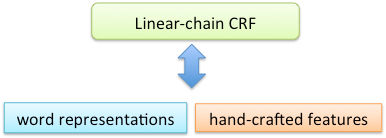
\includegraphics[scale = 0.3]{images/graph_transformer.png}
%   \caption{Architecture of linear-chain graph transformer}
%   \label{fig:graph_transformer}
% \end{figure}


As in~\newcite{turian2010word}, at each word position, we construct word
representation features from the words in a context window of size two
to either side of the target word, based on the pre-trained
representation of each word type.  For \brown, the features are the
prefix features extracted from word clusters in the same way
as~\newcite{turian2010word}. As a baseline, we include a one-hot
representation (which is equivalent to a linear-chain CRF with only
lexical context features).

Our hand-crafted features for \pos, \chunking and \mwe, are those used
by \newcite{collobert2011natural}, \newcite{turian2010word}
and~\newcite{mwecorpus}, respectively. For \ner, we use the same feature
space as \newcite{turian2010word}, except for the previous two
predictions, because we want to evaluate all word representations with
the same type of model -- a first-order graph transformer.

In training the distributed word representations, we consider two
settings: (1) the word representations are fixed during sequence model
training; and (2) the graph transformer fine-tunes the token-level word
representations during training.


\begin{table*}
\begin{small}
\begin{tabular}{cccccc}
\hline
			& \textbf{Training set} & \textbf{Validation set} & \textbf{\textit{In-domain} Test set} & \textbf{\textit{Out-of-domain} Test set} \\ \hline
\textbf{\pos} & \WSJ Sec.\ 0-18  & \WSJ Sec.\ 19--21 & \WSJ Sec.\ 22--24 & \EWT  \\
\textbf{\chunking} & \WSJ & \WSJ (1K sentences) & \CoNLLchunk & \Brown \\
\textbf{\ner} & \CoNLLner train set & \CoNLLner dev set & \CoNLLner test set & \MUC  \\
\textbf{\mwe} & \EWT (500 docs) & \EWT (100 docs)  & \EWT (123 docs) & --- \\
\hline
\end{tabular}
\caption{Dataset splits and feature space for each sequence labelling
  task.}
\label{datasplit}
\end{small}
\end{table*}


For each sequence labelling task, we experiment over the de facto
corpus, based on pre-existing training--dev--test splits where
available,\footnote{For the \mwe dataset, no such split pre-existed, so
  we constructed our own.} as follows:
\begin{itemize}
\item[\textbf{\pos}:] the Wall Street Journal portion of the Penn Treebank (\WSJ)
  with gold-standard Penn POS tags
\item[\textbf{\chunking}:] the Wall Street Journal portion of the Penn
  Treebank (\WSJ),
  converted into IOB-style full-text chunks using the CoNLL conversion
  scripts for training and dev, and the CoNLL-2000 full text chunking
  test data for testing
\item[\textbf{\ner}:] the CoNLL 2003 English Named Entity Recognition  Wall Street Journal
\item[\textbf{\mwe}:] the CoNLL Wall Street Journal
\end{itemize}
 For all tasks other
than \mwe,\footnote{Unfortunately, at the time of writing, there is no
  second domain which has been hand-tagged with MWEs using the method of
  \newcite{mwecorpus}, to use as an out-of-domain test corpus.} we
additionally have an out-of-domain test set, in order to evaluate the
out-of-domain robustness of the different word representations, with and
without fine-tuning. The \tabref{datasplit}

For fair and reproducible experimental results, we tuned the hyperparameters with random search~\cite{bergstra2012random}. 
We randomly sampled 50 distinct hyperparameter sets with the same random seed for the models that do not update word embeddings, and sampled 100 distinct hyperparameter sets for the models that do update word embeddings. 
For each set of hyperparameters, we train a model on its training set and choose the best one based on its performance on validation data~\cite{turian2010word}. 
We also tune the word representation hyperparameters -- namely, the word vector size and context window size (distributed representations) and the number of Brown clusters.
\nss{[Don't understand this sentence:]}This is achieved by mapping each possible hyperparameter combination to the word representation files trained with these parameters. 

\nss{[This paragraph needs work---I don't understand it:]}However, for the models that update word representations, we always found under-performed hyperparameters after trying out all hyperparameter combinations, because they have more hyperparameters than the models that do not update word representations. Then, for each distributed word representations, we reuse all hyperparameters of the models that do not update word representations, only tune the hyperparameters of AdaGrad for the word representation layer. This method requires only 32 additional runs for each model updating embeddings and achieves consistently better results than 100 random draws.

The final evaluation is carried out in a semi-supervised setting. We split the training set into 10 partitions at log scale (i.e., the second smallest partition will be twice the size of the smallest partition). We created 10 successively larger training sets by merging these partitions from the smallest one to the largest one, and \nss{(missing a verb?)} each of them on the same designated test sets. 

For easy comparison with previous results, we adopt the most widely used F1 measure as the evaluation metric for all tasks except POS-tagging, for which we use per-word accuracy. We also report model performance on out-of-vocabulary (unknown) words, i.e., the words that do not occur in the training set.

%\subsection{POS-tagging} We could choose one of the options. \subsubsection{Option 1} Almost the same setting as~\cite{collobert2011natural}, except adding one more test set.
% \noindent Training set: 0-18 of WSJ.
% \noindent Validation set: 19-21 of WSJ.
% \noindent Test set: 22-24 of WSJ, and English Web Treebank. We report model performances on these two test sets respectively.
% \noindent Feature space: the same set as in~\cite{collobert2011natural}

% \subsection{Chunking} The same setting as~\cite{turian2010word}\\
% \noindent Training set: WSJ train set.
% \noindent Validation set: Randomly sampled 1000 sentences from the train set for development.
% \noindent Test set: CoNLL2000 test set.
% \noindent Feature space: the same set as in~\cite{turian2010word}

% \subsection{MWE Identification} Training set: randomly sampled 500 documents from Nathana��s corpus. 
% \noindent Validation set: randomly sampled 100 documents from Nathana��s corpus.
% \noindent Test set: remaining 123 documents from Nathana��s corpus..
% \noindent Feature space: the same set as in~\cite{mwecorpus}

%\subsection{Named entity recognition} Training set: CoNLL03 train set.
% \noindent Validation set: CoNLL03 development set.
% \noindent Test set: CoNLL03 test set and MUC7. We report model performances on these two test sets respectively.
% \noindent Feature space: the same set as in~\cite{turian2010word}


%%% Local Variables: 
%%% mode: latex
%%% TeX-PDF-mode: t 
%%% TeX-master: "WordEmbEvaluation"
%%% End: 
